\section{Stand der Technik}
Die Fahrerlosen Transportsysteme und die Materialflusssysteme sind Prozesse der Logistik. In den vergangenen Jahren hat die Verbreitung Fahrerloser Transportsysteme (FTS) stark zugenommen. Beim Einsatz von FTS stellen sich vielfältige Konfigurierungs- und Planungsprobleme, so auch die Einsatzplanung f\"ur die einzelnen Fahrerlosen Transportfahrzeuge. (vgl. Günther; Krüger; Schrecker; 2000, S. 2). Der innerbetriebliche Materialfluss von Industrieunternehmen bietet fahrerlosen Transportsystemen (FTS) zahlreiche Einsatzgebiete: Sie verketten Produktionsprozesse, verknüpfen Fertigungsstationen oder ganze Betriebsbereiche und beschicken Montageplätze. Darüber hinaus dienen sie als mobile Werkbank oder versorgen und entsorgen Lager unterschiedlicher Art. Um die Systemvorteile von Fahrerlosen Transportsystemen und Materialflusssystemen zu optimieren, braucht man ein ma\ss gerechtes Wissen auf Ihr spezifisches Anlagekonzept abzustimmen. Wichtige Kriterien sind allerdings z.~B. die Einbindung der Fahrerlosen Transportsysteme in den gesamtbetrieblichen Materialfluss, die Anpassung an die vorhandenen Steuerungshierarchien und die optimale Auslegung der Technik in Bezug auf Fahrzeugbauart, Lastaufnahmemittel, Energiekonzept, Kommunikation und Leitsystem. (vgl. Werner Swoboda, Industrie Anzeiger). Ziele von Fahrerlosen Transportsystemen und Materialflusssystemen sind Kostensenkung durch Personaleinsparung, Verringerung von Transportsch\"aden, hohe Zuverl\"assigkeit in Vorg\"angen und bessere Materialflussplanung.
Dieses Kapitel wird in drei Teile gegliedert. Der erste Teil wird die Fahrerlosen Transportsysteme bzw die Orientierungs- und die Steuerungssysteme vorstellen und erkl\"aren; der zweite Teil ist eine Darstellung der Materialflusssysteme und ihrer verschiedenen Funktionen und der dritte Teil wird erkl\"aren, wie fahrerlose Transport- und Materialflusssysteme in gro\ss en Firmen wie Volkswagen und BMW Anwendung finden.

\subsection{Fahrerlose Transportsysteme}
Nach dem Verein Deutscher Ingenieure 2510 bestehen FTS im Wesentlichen aus "`einem oder mehreren Fahrerlosen Transportfahrzeugen (FTF), einer Leitsteuerung, Einrichtung zur Standortbestimmung und Lagererfassung, Einrichtungen zur Daten\"ubertragung sowie Infrastruktur und peripheren Einrichtungen"'. In seinem Buch Transport und Lagerlogistik fasst Martin die Definition von VDI 2510 eines FTS zusammen. Er beschreibt ein FTS als mit FTF ausgestattete rechnergesteuerte Materialflussanlagen zum automatischen Transport von G\"utern im innerbetrieblichen Materialfluss. (vgl. Martin H, 2006, S.262f). Bei FTS handelt es sich um flurgebundene F\"ordersysteme mit automatisch gef\"uhrten FTF. Die einzelnen FTF bef\"ordern Ladungstr\"ager zwischen zwei oder mehrere Stationen innerhalb eines Gebietes. Die Fahrzeugsteuerung erfolgt automatisch und rechnergest\"utzt. Der Einsatzbereich von FTS ist generell \"uberwiegend innerbetrieblich ausgerichtet. In diesen Rahmen \"ubernehmen FTS sowohl reine F\"orderaufgaben, wie Verkettung von Fertigungs- und Montageeinrichtungen als auch Aufgaben der Lagerbedienung und Kommissionierung. (vgl. G\"unther; Kr\"uger; Schrecker; 2000, S. 3). Das FTS ist eine Technik, die im Vergleich gegen\"uber Stetigf\"ordersystemen eine hohe Anpassungsf\"ahigkeit an die sich \"andernden Marktsituationen zum Vorteil hat. Daher konzentrieren die Forschungs- und Entwicklungsaktivit\"aten sich heutzutage auf die sog. „Zellul\"aren F\"ordersysteme“, in welchen stetige F\"orderanlagen zur Verkn\"upfung von Logistischen Funktionen durch individuelle, autonom arbeitende FTF ersetzt werden (vgl. Ten Hompel; Heidenblut, 2008). Die Haupteinsatzgebiete des FTS liegen nun in der Intralogistik. Also bei der Organisation, der Steuerung, der Durchf\"uhrung und der Optimierung des innerbetrieblichen Waren- und Materialflusses und Logistik, der Informationsstr\"ome sowie des Warenumschlags in Industrie, Handel und \"offentlichen Einrichtungen. Z.~B. Automobil- und Zulieferindustrie, Papiererzeugung und –verarbeitung, Elektroindustrie, Getr\"anke-, Lebensmittelindustrie, Baustoffe, Stahlindustrie, Kliniklogistik (G\"unter Ullrich, 2011 S. 13). FTS bestehen im Wesentlichen aus drei Systemkomponenten: Die Fahrerlosen Transportfahrzeuge, das Orientierungssystem, das Steuerungssystem. 

\subsection{Fahrerlose Transportfahrzeuge}
Die FTF sind flurgebundene F\"ordermittel mit eigenem Fahrantrieb, die automatisch gef\"uhrt, gesteuert und ber\"uhrungslos gef\"uhrt werden. Sie dienen dem Materialtransport, und zwar zum Ziehen und/oder Tragen von F\"ordergut mit aktiven oder passiven (FTF mit passiver Lastaufnahme werden von anderen F\"ordermitteln gezogen oder manuell mit den G\"utern best\"uckt) Lastaufnahmemittel (VDI 2510). Da das FTS mit fahrerlosen Aspekten systematisiert ist, ergeben sich dann auf der funktionalen Ebene Unterschiede zu fahrerbedienten Fahrzeugen, wie z.~B. den klassischen Gabelstaplern und FTF. Im Rahmen dieser Arbeit wird nur auf eine Kategorie von FTF tiefer eingegangen: das Mini-FTF. Die Mini-FTF sind kleine, schnelle, intelligente und flexible Fahrzeuge, die extrem schnell Bed\"urfnisse befriedigen k\"onnen. Heutzutage arbeiten viele Universit\"aten in der ganzen Welt im Bereich der Schwarm-Experimente. Hier sollen die kleinen FTF intelligent miteinander arbeiten. Die Fahrzeuge sollen sich ohne eine eigene separate FTS-Leitsteuerung untereinander verst\"andigen, Strategien entwickeln und gemeinsam Arbeiten ausf\"uhren. Die Forschungsgebiete hei\"ssen Agentensysteme und Schwarmtheorie. Die Mini-FTF k\"onnen nur intralogistische Aufgaben ausf\"uhren. Dennoch sind viele unkonventionelle Einsatzf\"alle denkbar. Die Kommissionierung (eine ausf\"uhrliche Begriffserkl\"arung wird im Teil Materialfluss gegeben) ist die verbreitetste Anwendungsm\"oglichkeit von Mini-FTF (G\"unter Ullrich, 2011 S. 105).
Als Zusammenfassung kann man sagen, dass die Fahrzeugsteuerung die Systemsicherheit, das Energiemanagement, das Lastaufnahmemittel und die Lenkung eines FTF gew\"ahrleistet. Ein FTF kann ohne Energie nicht funktionieren. Damit ein FTF seine Aufgabe erf\"ullen kann, ist eine Energieversorgung notwendig. Die FTF können durch Akkus oder Traktionsbatterien oder mit Hilfe eines Induktionssystems oder einer Stromschiene mit Energie versorgt werden. Jedoch k\"onnen die beiden Versorgungsarten gekoppelt werden, um ein Hybridsystem zu bekommen. Die Notwendigkeit der Existenz einer Ladestation in einem FTS ist unumstritten. Die FTF m\"ussen immer mit Energie versorgt werden. Je nachdem wie die FTF programmiert sind, kann ein FTF bei Energiebedarf selber zur Ladestation fahren oder von einem Auftraggeber (Mensch) zur Ladestation gef\"uhrt werden.

\subsubsection{Orientierungssystem bzw. Navigation}
Das Orientierungssystem bzw. die Navigation dient zur Lokalisierung des Fahrzeugs. Sie ist ein Hilfsmittel zur Berechnung des sichersten Wegs, um das Ziel zu erreichen. Au\ss erdem dient die Navigation auch zur Vermeidung von eventuellen Kollisionen. Sie gilt sowohl f\"ur die Orientierung als auch f\"ur die Sicherheit des Fahrzeuges und seines Umfeldes. W\"ahrend seiner Bewegung bzw. Orientierung folgt das FTF einer physischen oder virtuellen Linie (Spur), damit es sein Ziel gefahrlos erreichen kann. Aufgrund eines Sicherheitssystems sollte das FTF bei Kollisionsgefahr oder wenn Hindernisse vor ihm stehen, sofort anhalten. 
Unter Navigationshilfe versteht man nicht nur die Positionierung und Orientierung des Fahrzeuges sondern auch, wohin das Fahrzeug gelangen w\"urde, wenn keine auf seine Bewegung ver\"andernden Ma\ss nahmen ergriffen würden.
Die Steuerung sagt, was zu tun ist, und die Navigation bestimmt, auf welchem Weg das gew\"unschte Ziel sicher zu erreichen ist bzw. ob das FTF einen vorgegebenen Weg weiter verfolgen oder einen alternative Weg nehmen soll.
Die Steuerung von fahrerlosen Transportfahrzeugen, deren Grundfunktionen und der Umgang mit diesen werden in den VDI-Richtlinien [VDI92], [VDI94], [VDI04] vorgestellt.
F\"ur das Konstrukt der fahrerlosen Transportsysteme werden verschiedene Ans\"atze verfolgt, die abh\"angig vom System verschiedene Konstruktionsbem\"uhungen auf das Fahrzeug oder auf der Strecke erfordern.
Es gibt mehrere Navigationsverfahren: die physische Leitlinie, die Orientierung durch Magnetmarken, das Global Positioning System (GPS) und die Lasernavigation (vgl. G\"unter Ullrich, 2011 S. 112).
\begin{itemize}
	\item \textbf{Die physische Leitlinie:}  Fahrerlose Transportsysteme, die auf physischen Leitlinien navigieren bzw. fahren, benutzen Einrichtungen am oder im Fu\ss boden. Die verschiedenen Varianten sind:
 \item \textbf{Orientierung durch optische Leitspur:} Bei dieser Methode wird ein Farbstrich mit deutlichem Farbkontrast zum umgebenden Boden entweder lackiert oder mit einem speziellen Gewebeband aufgebracht.
Eine geeignete Kamerasensorik unter dem Fahrzeug nutzt Kantendetektions-Algorithmen und errechnet so die Ansteuerungssignale f\"ur den Lenkmotor (G\"unter Ullrich, 2011 S. 112).
Optische Verfahren dienen durch eine st\"andige Kurskorrektur dazu, eine hohe Fahrgenauigkeit zu erreichen. 
\item \textbf{Orientierung durch induktive Leitspur:} Diese Methode der Navigation fahrerloser Transportfahrzeuge ist profitabel aufgrund der permanenten Kurskorrektur und au\ss erdem besonders zuverl\"assig und fahrzeugseitig durch die Nutzung einfacher Komponente zu realisieren.
Es ist m\"oglich, die Stromversorgung der Fahrzeuge fahrbahnseitig zu realisieren, sodass die Nutzung schwerer Akkumulatoren entf\"allt.
Jedoch sind Systeme mit Leitdrahtsteuerung nicht flexibel und in der Konstruktion sehr teuer.
\begin{figure}[h!]
	\centering
		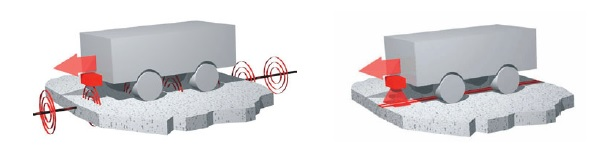
\includegraphics[width=0.9\textwidth]{Prinzipskizze_induktiven.jpg}
	\caption{Prinzipskizze zur induktiven und optischen Spurf\"uhrung (Quelle: G\"unter Ullrich, 2011 S. 79)}
	\label{Prinzipskizze_induktiven}
\end{figure}  
	\item \textbf{Orientierung durch Magnetmarken:} Eine weitere M\"oglichkeit der Steuerung ist die Abtastung von Magnetstreifen oder magnetischen Markierungen auf der Straßenoberfl\"ache.
Dabei bedarf es zur Berechnung der Leitlinie entweder der Koppelnavigation, oder der Peilung von in regelm\"a\ss igen Abst\"anden in den Boden eingelassenen Marken.
Diese Marken k\"onnen rein passive Dauermagnete oder aber quasi-aktive Transponder sein (G\"unter Ullrich, 2011 S. 80).
Das Bild \ref{Prinzipskizze_Koppelnavigation_rechts} ist eine Repr\"asentation der Navigation durch Magnetstreifen.
	\begin{figure}[h!]
		\centering
			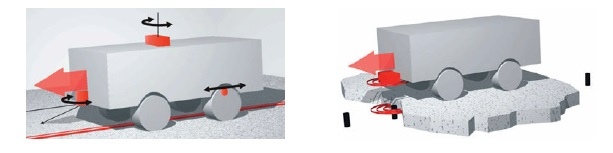
\includegraphics[width=0.9\textwidth]{Prinzipskizze_Koppelnavigation_rechts.jpg}
			\caption{Prinzipskizze zur Koppelnavigation (links) und zur Magnet- bzw. Transpondernavigation (rechts) (Quelle: G\"unter Ullrich, 2011 S. 79)}
			\label{Prinzipskizze_Koppelnavigation_rechts}
	\end{figure}	
	\item Bei der Lasernavigation bestimmt der Laserscanner die Position des FTF, dazu kommen noch optische Sensoren f\"ur die Erkennung von Hindernissen wie z.~B. Menschen.
Lasergef\"uhrte FTS bieten einen hohen Wert an Flexibilit\"at, da sie ohne Bodeninstallation funktionieren.
Nur bei engerem Raum kann die Lasernavigation nicht so effizient wie z.~B. eine induktive Spurf\"uhrung sein, wenn viele Fahrzeuge zum Einsatz kommen.
Um die Systemvorteile einer Lasernavigation optimal zu nutzen, ben\"otigt man allerdings ein passendes Anlagenkonzept.
Die wichtigsten Kriterien sind: die Einbindung in das gesamtbetriebliche Materialflusssystem, die Anpassung an die vorhandenen Steuerungshierarchien und die optimale Auslegung der Technik in Bezug auf Fahrzeugbauart, Lastaufnahmemittel, Energiekonzept, Kommunikation und Leitsystem.
Ein Aspekt, der f\"ur das Laser-gef\"uhrte FTS spricht, ist die Wirtschaftlichkeit.
Und dies trotz der Alternativen Elektro-, Low-Cost- sowie induktiv gef\"uhrten FTS.
Letztere lassen sich so einrichten, dass sie auch auf leitdrahtlosen, rein rechnergef\"uhrten Teilstrecken verkehren k\"onnen.
Keinerlei kostenintensive Bodeninstallation ben\"otigt dagegen das \"uber Lasersensor gesteuerte, v\"ollig frei navigierende Laser-FTS.
Die Fahrzeuge orientieren sich lediglich an im Raum verteilten Reflektoren und mit Hilfe der Kombination von Winkel- und Distanzmessung. (Werner Swoboda, Industrie Anzeiger). Das Bild \ref{Prinzipskizze_Koppelnavigation_links} ist eine Visualisierung der Lasernavigation.
	\begin{figure}[h!]
		\centering
		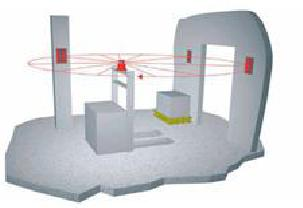
\includegraphics[width=0.8\textwidth]{Prinzipskizze_Koppelnavigation_links.jpg}
		\caption{Prinzipskizze zur Koppelnavigation (links) und zur Magnet- bzw. Transpondernavigation (rechts) (Quelle: G\"unter Ullrich, 2011 S. 79)}
		\label{Prinzipskizze_Koppelnavigation_links}
	\end{figure}

	\item \textbf{Orientierung durch GPS:} Seine Anwendung im Bereich der Fahrzeugsteuerung wird in Form des DGPS eingesetzt.
DGPS bedeutet differential GPS und meint die Verwendung eines zus\"atzlichen GPS-Empf\"angers, der nicht auf dem FTF, sondern station\"ar fest installiert ist.
Mit Hilfe dieses ortsfesten GPS-Empf\"angers wird der sich zeitlich \"andernde Fehler ermittelt, der dem GPS-System eigen ist.
Mit Hilfe dieser Kenntnis k\"onnen zeitgleich die fahrenden GPS-Empf\"anger auf den FTF exakte Positionen ermitteln (Quelle: G\"unter Ullrich, 2011 S. 27).
Diese Navigationstechnik benötigt einen freie Sichtkegel von 15 Grad nach oben (siehe Bild 4), um zuverl\"assig arbeiten zu k\"onnen.
Die Schritte zur Erlangung der erforderlichen Fahr- und Positioniergenauigkeit sind:
	\begin{itemize}
		\item Pr\"ufung der \"ortlichen Gegebenheiten, insb. der Empfangsst\"arken der Satelliten
 \item Einsatz des Differential-GPS
 \item Real Time Kinematic Differential GPS. 
\end{itemize}
	\begin{figure}[h!]
		\centering
		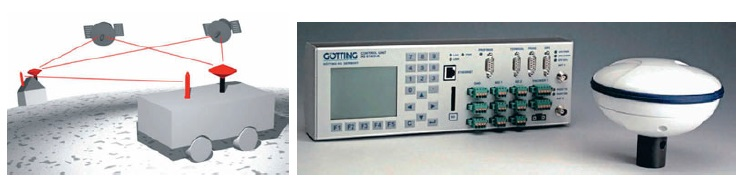
\includegraphics[width=0.9\textwidth]{Prinzipskizze_zur_Navigation_mittels_GPS.jpg}
		\caption{Prinzipskizze zur Koppelnavigation (links) und zur Magnet- bzw. Transpondernavigation (rechts) (Quelle: G\"unter Ullrich, 2011 S. 79)}
		\label{Systemarchitektur_FTS}
\end{figure}
Im Rahmen des Projekt FAISE wird die Navigation durch den Laser durchgef\"uhrt. Es kann hier kein Global Positioning System (GPS) verwendet werden, da das ganze Experiment in einem geschlossenen Raum gemacht wird.
Weiterhin wird auch keine Navigation durch die physische Leitlinie oder durch die St\"utzpunkte im Boden erzielt, weil dazu der Boden gebrochen werden m\"usste.
\end{itemize}

\subsubsection{Steuerungstechnik}
Die interne Materialflusssteuerung ist eine Vorstufe der Transportauftragsabwicklung und wird nur dann ben\"otigt, wenn die Transportauftr\"age nicht klar dezidiert \"ubertragen, sondern aufbereitet werden m\"ussen. Eine Anforderung wie z. B. ben\"otige Ware A an Maschine B erfordert eine Umsetzung in einen oder mehrere Transportauftr\"age nach dem klassischen Muster. Hole von C und Bringe nach D. Die FTS-interne Materialflusssteuerung kombiniert also Quelle und Senke \"uber die in ihr hinterlegten Transportbeziehungen zu einem Transportauftrag und schickt diesen zur Durchf\"uhrung an die Transportauftragsverwaltung. Diese ganze Transportauftragsverwaltung ist in der FTS-Leisteuerung geregelt. 
Die FTS-Leitsteuerung ist die Kommandozentrale, um das FTS in das Umfeld zu integrieren. Au\"sserdem steuert es die FTF, die sich im System befinden. Damit ist das FTS dann in der 
Lage, die ihm \"ubertragenen Auftr\"age zu erf\"ullen. "`Eine FTS-Leitsteuerung besteht aus Hard- und Software. Kern ist ein Computerprogramm, das auf einem oder mehreren Rechnern abl\"auft. Sie dient der Koordination mehrerer Fahrerloser Transportfahrzeuge und/oder \"ubernimmt die Integration des FTS in die innerbetrieblichen Abl\"aufe."' (VDI 4451). Die Leitsteuerung bringt das FTS in seinem Umfeld zusammen, bietet seinen Bedienern vielf\"altige Service-M\"oglichkeiten und nimmt Transportauftr\"age entgegen. Weiterhin stellt sie den Aufgaben entsprechende Funktionsbl\"ocke zur Verf\"ugung. 
Die FTS-Leitsteuerung ist der Kern der FTS. In Rahmen des Projekt FAISE, wird es auch eine Leisteuerung ben\"otigt. Eine Leitsteuerung ist nur mit Hilfe eine Systemarchitektur zu implementieren und zu verstehen. In seinem Buch Fahrerlose Transportsysteme, hat G\"unter Ulrich zwei verschiedene Systemarchitekturen dargestellt. Eine f\"ur eine einfache FTS und eine andere f\"ur eine komplexe FTS. Da es bei FAISE nur mit vier FTF gearbeitet wird, ist es sinnvoll mit einer einfachen Systemarchitektur zu arbeiten. Das Bild 3 ist eine Repr\"asentation einer einfachen Systemarchitektur.
	\begin{figure}[h!]
		\centering
		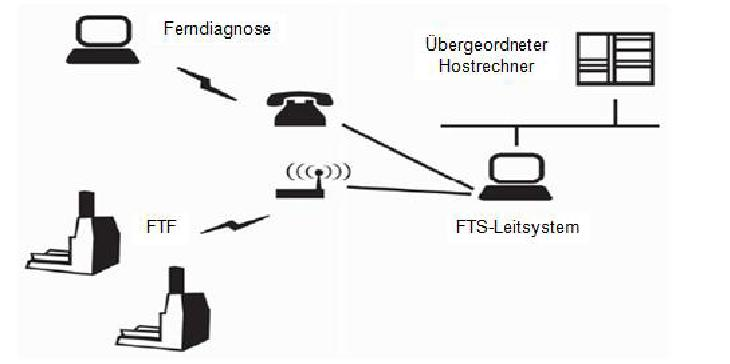
\includegraphics[width=0.9\textwidth]{Systemarchitektur_FTS.jpg}
		\caption{Die Systemarchitektur eines einfachen FTS (Quelle: G\"unter Ullrich, 2011 S. 93)}
		\label{Systemarchitektur_FTS}
	\end{figure}

Es gibt eine geringe Anzahl von FTF, mit denen die Leitsteuerung per WLAN in Verbindung ist. Au\"sserdem gibt es ein LAN, \"uber das es eine direkte Verbindung mit einem \"ubergeordneten Rechner gibt, von dem die Transportauftr\"age kommen. \"uber die angedeutete Telefonleitung ist eine VPN-Verbindung zur Ferndiagnose eingerichtet. Die Daten\"ubertragung zu den \"ubergeordneten Host-Rechnern erfolgt meist \"uber lokale, Ethernet basierte Netzwerke mit dem Protokoll TCP/IP. Solche Host-Rechner k\"onnen beispielweise Materialflusssteuerungssysteme zur Produktionssteuerung (z. B. SAP) Produktionsplanungssysteme (PPS) Lagerverwaltungssysteme (LVS) sein.“( vgl. G\"unter Ullrich, 2011 S. 96). 
Au\"sserdem nach der VDI 4451(Blatt 3) „zum internen Umfeld der FTF-Steuerung geh\"oren das Lastaufnahmemittel (LAM), Sensoren und Aktoren, Bedienfeld am Fahrzeug und das Sicherheitssystem. Das externe Umfeld besteht aus der FTS-Leisteuerung, anderen FTF, automatischen Stationen und Geb\"audeeinrichtungen“. Die Abbildung 1 stellt eine Darstellung eine FTF-Steuerung und ihr Steuerungsumfeld dar.
	\begin{figure}[h!]
		\centering
		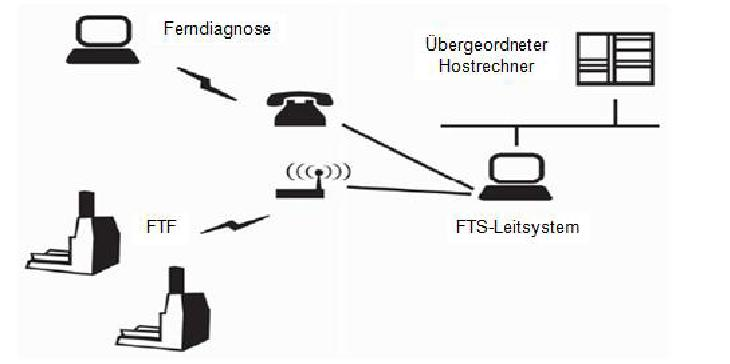
\includegraphics[width=0.9\textwidth]{Systemarchitektur_FTS.jpg}
		\caption{Allgemeine Darstellung einer FTF-Steuerung mit Datenschnittstellen (vgl. VDI 4451)}
		\label{Wertschoepfungskette}
	\end{figure}
Die administrative Ebene, die h\"aufig \"uber einen station\"aren Leitrechner realisiert wird, verwaltet die Transportauftr\"age der ganzen Materialflusssteuerung. Die operative Ebene, die auch als Fahrzeugsteuerung bezeichnet wird, erh\"alt ihre Informationen \"uber die Fahrzeugdisposition der administrativen Ebene. Der Funktionsblock Kommunikation leitet den stattgefundenen Datenaustausch zum Manager weiter. Dieser sorgt f\"ur die Koordination, indem er die Fahrauftr\"age in einzelne Befehle aufteilt, sowie f\"ur ein reibungsloses Zusammenwirken der einzelnen Funktionsbl\"ocke. Neben dem Block Kommunikation sind weitere Bl\"ocke vorhanden. Dazu geh\"ort f\"ur die gesamte Last\"ubergabe inklusive der Lastlagererfassung verantwortliche Lastaufnahme, das Energiemanagement, welches den Lade- und Allgemeinzustand der Batterien \"uberwacht, und der Block \"uberwachung/Sicherheitsschnittstelle, welcher zum Schutz der Personen und Sachgegenst\"ande dient. Der Funktionsblock Fahren und die damit verbundene Sensorik bzw. Aktorik koordinieren die Ablaufsteuerung der Funktionen des Orientierungssystems (Langenbach Maik, 2012, S. 33).

\subsection{Materialflusssysteme}
Damit ein Produkt auf den Markt kommen kann, muss man ihn denken, ihn erstellen und dann ihn vermarken. Die Produkterstellung und -vermarktung sind Prozesse des Wirtschaftens. Vorprodukte oder Materialen werden von Beschaffungsm\"arkten in die Unternehmen gef\"uhrt und dort werden sie durch besondere Produktionsprozesse transformiert. Am Ende der Produktion, steht ein Endprodukt, der f\"ur den Konsum bereits ist. 
Die Produktion und Logistik von G\"utern sind daher sehr wichtige Bereiche f\"ur den Unternehmenserfolg. Allerdings f\"uhren heute die unterschiedlichen Auspr\"agungen der Logistik z.B. in Produktions-, Handels-, oder Verkehrsunternehmen zu einer terminologischen Differenzierung der Logistik. Der Materialflussbegriff leitet sich einfach von dem logistische Konzept ab, in anderen W\"ortern das Materialflusssystem f\"uhrt in der Logistik zur\"uck. Die Abbildung 2. dient zur Erl\"auterung einer konventionellen Wertsch\"opfungskette. 
	\begin{figure}[h!]
		\centering
		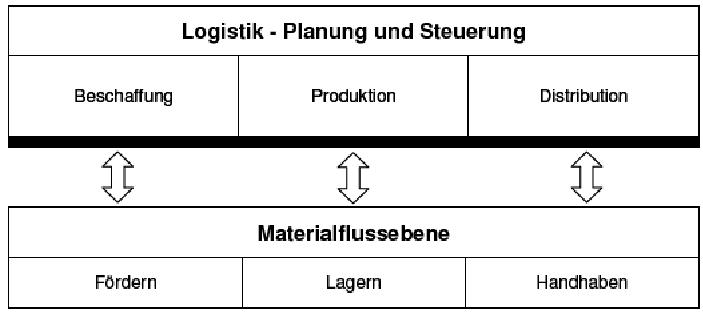
\includegraphics[width=0.9\textwidth]{Wertschoepfungskette.jpg}
	\caption{Elemente einer Wertsch\"opfungskette (vgl. Wulz, J, 2008, S. 7)}
	\label{Wertschoepfungskette}
\end{figure}

Der Begriff Materialfluss bedeutet die Verkettung aller Prozesse bei der Beschaffung, Bearbeitung, Verarbeitung sowie bei der Distribution von G\"utern innerhalb festgelegter Bereiche. Deswegen l\"asst sich der Materialfluss in vier Stufen unterordnet: externer Transport, betriebsinterner Materialfluss, geb\"audeinterner Materialfluss und Materialfluss am Arbeitsplatz. Nach dem Verein Deutscher Ingenieur bzw. VDI-241 beinhaltet die Logistik f\"unf Hauptfunktionen. Diese Funktionen sind Bearbeiten, Pr\"ufen, Handhaben, F\"ordern, Lagern und Aufenthalten. Neben diesen Hauptfunktionen z\"ahlen auch Nebenfunktionen wie z.B. Montieren, Umschlagen, Kommissionieren, Palettieren und Verpacken (VDI 2411). Jedoch ist auf der Ebene des Materialflusssystems nur drei Funktionen zu ber\"ucksichtigen: F\"ordern, Lagern, Handhaben. Die anderen Funktionen setzen sich normalerweise aus den erl\"auterten Funktionen zusammen. Dieses Arbeitsteil wird in zwei Teile gegliedert. Im ersten Teil werden die drei Funktionen der Materialflusssysteme vorgestellt Im zweiten Teil wird eine Planung von Materialflusssystemen dargestellt.

\paragraph{Funktionen von Materialflusssystemen}
\begin{itemize}
	\item \textbf{Funktion F\"ordern} \\
	F\"ordern bedeutet Transportieren und ist eine der wichtigsten Aspekte innerhalb des Materialflusssystems. Nach der VDI 2411 ist F\"ordern das Fortbewegen von Arbeitsgegenst\"anden in einem System. „Die Fortbewegung oder Ortver\"anderung von G\"utern oder Personen mit technischen Mitteln wird allgemein als Transport bezeichnet. Findet diese Ortsver\"anderung in einem r\"aumlich begrenzten Gebiet wie beispielsweise innerhalb eines Betriebes oder Werkes statt, so wird dieser Vorgang durch den Begriff F\"ordern pr\"azisiert. Das F\"ordern bzw. die F\"ordertechnik umfasst also das Bewegen von G\"utern und Personen \"uber relativ kurze Entfernungen einschlie\"sslich der dazu notwendigen technischen organisatorischen und personellen Mittel“(Ten Hompel, Schmidt, Nagel, 2007, S. 119). 
Das F\"ordermittel (technisches Transportmittel, zur Ortsver\"anderung von G\"utern oder Personen) und das F\"orderelement bilden das physikalische Bestandteil eines F\"ordervorgang. Der Ablauf und die Steuerung werden durch den F\"ordervorgang dargestellt. In Punkto F\"ordermittel kann auf verschiedenste Elemente der Materialflusstechnik zur\"uckgegriffen werden. Dies umfasst unter anderen Rollenbahnen, und FTS. Neben der M\"oglichkeit auf automatisierte F\"ordermittel zur\"uckzugreifen, kommen auch manuell mechanisierte bzw. rein manuelle Systeme zum Einsatz. In diesem Fall ist der Mensch oder der Bediener eines F\"ordermittels wesentlich f\"ur den Ablauf eines reibungslosen Materialflusses in Zusammenspiel mit den physikalischen Elementen sowie dem Prozessablauf verantwortlich. (Wulz, J, 2008, S. 8). Das Bild 4 gilt als Beispiel eines F\"ordersystems. 
	\begin{figure}[h!]
	\centering
  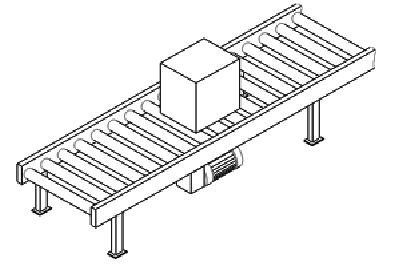
\includegraphics[width=0.7\textwidth]{Stetigfoerderer.jpg}
	\caption{Beispiel eines Stetigf\"orderer (entnommen aus Ten Hompel, Schmidt, Nagel, 2007, S. 131)}
	\label{Stetigfoerderer}
\end{figure}

\item \textbf{Funktion Lagern} \\
Das Lagern ist jedes geplante Liegen des Arbeitsgegenstandes im Materialfluss. Das Lager ist ein r\"aumlich abgegrenzter Bereich bzw. eine Fl\"ache zum Aufbewahren von St\"uck- und/oder Sch\"uttg\"utern in Form von Rohmaterialien, Zwischenprodukte oder Endprodukte, das mengenm\"a\"ssig erfasst wird (VDI-2411). Die Einlagerung von Lagereinheiten, die Aufbewahrung und Bereithaltung von Lagereinheiten auf Lagerpl\"atzen und die Auslagerung einer Lagereinheit, sind die grundlegenden Prozesse in einem Lager.
Aufgrund der starken Ver\"anderungen im Markt, m\"ussen auch die unternehmerischen Abl\"aufe an Lagersysteme schnell angepasst werden. In einem Lagersystem werden im Verlauf des Materialflusses Speicher- bzw. Lagerfunktionen sowie F\"orderfunktionen wahrgenommen. 
Aufgabe eines Lagers ist das Bevorraten, Puffern und Verteilen von G\"utern. W\"ahrend Vorratslager lang- und mittelfristige und Pufferlager kurzfristige Bedarfsschwankungen ausgleichen sollen, erf\"ullen Verteillager neben der Bevorratungs- noch eine Kommissionierfunktion. Daher k\"onnen die Aufgaben eines Lagers anhand folgender Ausgleichsma\"ssnahmen beschrieben werden: Zeitausgleich, Mengenausgleich, Raumausgleich und Sortimentsausgleich. (Stich, V.; Bruckner, A.; 2002). Ein Zeitausgleich ist immer dann erforderlich, wenn die Zeitfunktion der Nachfrage nicht der Zeitfunktion der Produktion entspricht. Beispielsweise steht eine losgr\"o\"ssenoptimierte Fertigung einer saisonalen Nachfrage gegen\"uber. Gerade in Bereichen mit Serienfertigung, in denen aus Kostengr\"unden in der Regel gr\"o\"ssere Mengen als die Nachfragemengen produziert werden, muss Mengenausgleich vollzogen werden. Sobald der Produktionsort nicht mit dem des Produktabnehmers \"ubereinstimmt, findet mit Hilfe von Verkehrstr\"agern ein Raumausgleich statt. Mit zunehmender Sortimentsbreite steigt die Wahrscheinlichkeit, dass die Anzahl der Produktionsstandardorte steigt. (Lagenbach, M, 2012, S. 14).

\item \textbf{Funktion Handhaben } \\
Der Begriff Handhaben wurde gedanklich von de menschlichen Hand abgeleitet, wird aber auch f\"ur automatische ablaufende Vorg\"ange zur Manipulation von Objekten gebraucht. Handhaben bedeutet etwas greifen, bewegen und an einem bestimmten Ort ablegen. Das hei\"sst, durch Handhaben wird die Lage oder Position von Objekten ge\"andert. Im \"ubertragenen Sinne bedeutet handhaben auch bewerkstelligen bzw. praktisch aus\"uben. Von Handhabungstechnik spricht man, wenn f\"ur die Handhabung Ger\"ate eingesetzt werden. 
Die Richtline VDI 2860 definiert die Funktion Handhaben als „das Schaffen, definiertes Ver\"andern oder vor\"ubergehendes Aufrechterhalten einer vorgegebenen r\"aumlichen Anordnung von geometrisch bestimmten K\"orpern.“ Die Teilfunktionen des Handhabens stellen das Speichern, das Bewegen, das Sichern, das Kontrollieren und das Ver\"andern von G\"utern dar. Das Handhaben kann sowohl als eine Funktion als auch eine Fertigung des Materialflusses betrachtet werden. Eine m\"ogliche Handhabungsfunktion im Materialfluss ist z.B. das Palettieren, worunter die Stapelung von St\"uckg\"utern zu einem St\"uckgutstapel nach einem gewissen Muster verstanden wird. Handhabungsfunktionen k\"onnen entweder von Automaten z.B. Roboter oder von Menschen durchgef\"uhrt werden. Auf Grund der Greifflexibilit\"at ist der Mensch jedoch meist un\"ubertroffen in der Handhabung.
\end{itemize}

\subsection{Fallbeispiele}
\subsubsection{FTS in der Gl\"asernen Manufaktur Dresden (Volkswagen)}
Volkswagen AG montiert das neue Modell der Luxusklasse "Phaeton" in der "Gl\"asernen Manufaktur" in Dresden. Die Materialversorgung \"ubernimmt ein fahrerloses Transportsystem mit 56 frei navigierenden Fahrzeugen. Die gesamte Steuerungs- und Navigationstechnik stammt von FROG Navigation Systems, dem Projektpartner des Generalunternehmers AFT (Mechanik).
Die Produktion ist auf drei Ebenen unterteilt: . Die eigentliche Montage findet auf den beiden oberen Montageebenen statt: Die Rohrkarosse befindet sich auf einer Montageplattform, die Teil des Schuppenbandes ist, das sich sicher in den Hallenboden einf\"ugt und mit konstanter Geschwindigkeit durch die Montagezyklen bewegt. Danach erfolgt die \"ubergabe an eine schwere Elektroh\"angebahn (EHB) zur H\"angemontage. W\"ahrend der H\"angemontage erfolgt die Hochzeit, d. h. das Zusammenf\"ugen von Karosse und Triebsatz, wobei der Triebsatz von einem Fahrerlosen Transportfahrzeug (FTF) herangebracht wird. Anschlie\"ssend wird die Karosse wieder auf eine Schubplattform, die sog Schuppe, zur Komplettierung und Qualit\"atskontrolle gestellt.

Im Untergeschoss, der Logistikebene, wird die verbauende Ausr\"ustung zur Verf\"ugung gestellt und in Betrieb genommen. Die FTS \"uberminnt die Versorgungsleitungen der Materialien und damit eine erhebliche logistische Funktion . Um zwischen den Ebenen zu wechseln, nutzen die  automatischen Fahrzeug-Hebeb\"uhnen .
Das FTS hat die grunds\"atzliche Aufgabe, die Montagelinien (Schuppenband oder EHB) zu versorgen. Dabei wird allerdings zwischen folgenden sechs Gewerken unterschieden:
\begin{itemize}
\item[1.] Anlieferung von Warenk\"orben auf die Schuppe
\item[2.] Anlieferung von Schalttafeln (Cockpits)
\item[3.] Anlieferung von Kabelstr\"angen
\item[4.] Anlieferung des Triebwerks mit Fahrwerk und Ausf\"uhrung der Hochzeit
\item[5.] Anlieferung von Warenk\"orben zur H\"angemontage
\item[6.] Anlieferung der T\"uren plus Warenk\"orbe
\end{itemize}
\subsubsection{FTS beim Automobilhersteller BMW im Werk Leipzig}
Das BMW-Werk in Leipzig hat im Jahre 2005 mit der Produktion der 3er reihe (E90) gestartet
Im Bereich der Teileversorgung \"ubernimmt erstmals in der Geschichte der Automobilindustrie ein Fahrerloses Transportsystem (FTS) umfangreiche Logistikfunktionen. Folgende Prozesse wurde f\"ur die Teilversorgung im Leipzig-Werk definiert:

\begin{itemize}
\item Direktanlieferung per LKW: Gro\"sse Teile mit geringer Komplexit\"at (z. B. Bodenmatte oder Kofferraumverkleidung) werden per LKW zeitnah und in unmittelbare N\"ahe des Verbauortes angeliefert.
\item Modulanlieferung per EHB8: Gro\"sse und komplexe Baugruppen (z. B. Cockpit) werden direkt auf dem Werksgel\"ande von externen Lieferanten oder BMW Mitarbeitern montiert.
\item Lagerware per FTS: Die Mehrzahl der Teile wird in einem Versorgungszentrum gelagert, kommissioniert und mit Fahrerlosen Transportfahrzeugen (FTF) an die jeweiligen Verbauorte in der Montage gebracht (G\"unter Ullrich, 2011 S. 36).\end{itemize}
Es sind 74 FTF im Einsatz, als Ladehilfsmittel werden mehr als 2.000 Rollwagen in zwei unterschiedlichen Ausf\"uhrungen eingesetzt. Je FTF werden entweder zwei kleine Rollwagen, zur Aufnahme von Beh\"altern bis DIN-Gr\"o\"sse, oder ein so genannter \"ubergro\"sser Rollwagen zur Aufnahme von Gro\"ssbeh\"altern eingesetzt. Zus\"atzlich gibt es noch die Sequenziergestelle mit Sonderaufbauten (G\"unter Ullrich, 2011 S. 37). Durch einen Laser-Scanner auf dem FTF wird den Personenschutz und Hinderniserkennung \"ubernommen. 

Die Fahrerlosen Transportfahrzeuge finden ihren Weg mit Hilfe der so genannten freien Navigation. Damit ist gemeint, das die Fahrzeuge ohne physikalische Leitspuren und nach einem kombinierten Prinzip aus Kopplung und Peilung arbeiten. Kopplung bedeutet die Auswertung von fahrzeuginternen Sensoren (Messr\"ader und ein faseroptischer Kreisel), wodurch der zur\"uckgelegte Weg samt Kurven bestimmt wird (G\"unter Ullrich, 2011 S. 37). Bei jeder Peilung werden aufgetretene Fahrfehler, die durch Schlupf der R\"ader oder durch Ver\"anderungen des Raddurchmessers auftreten k\"onnen, korrigiert. Die Vorteile dieses, auch Magnet Navigation genannten, Verfahrens liegen in der Zuverl\"assigkeit und der Flexibilit\"at bei zuk\"unftigen Layoutanpassungen (G\"unter Ullrich, 2011 S. 37).


